\documentclass{standalone}
\usepackage{ tikz }
\usepackage{ xparse }
\usepackage{ amssymb }
\usepackage{../../macros}

\begin{document}
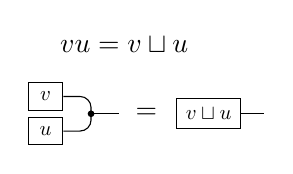
\begin{tikzpicture}[yscale=-1,x=1em,y=1.25em]

    \node at (2.2,-2) {$v \tensor u \seq \join = v \sqcup u$};

    \node [draw, minimum width=1.25em, minimum height=1em, anchor=east] at (0,-0.5) {\scalebox{0.75}{$v$}};
    \node [draw, minimum width=1.25em, minimum height=1em, anchor=east] at (0,0.5) {\scalebox{0.75}{$u$}};

    \draw [rounded corners] (0,-0.5) -- (1,-0.5) -- (1,0);
    \draw [rounded corners]  (0,0.5) -- (1,0.5) -- (1,0);
    \filldraw (1,0) circle (1pt);
    \draw (1,0) -- (2,0);

    \node at (3,0) {$=$};

    \node [draw, minimum width=1em, minimum height=1em] at (5.25,0) {\scalebox{0.75}{$v \sqcup u$}};
    \draw (6.4,0) -- (7.25,0);

\end{tikzpicture}
\end{document}